\documentclass[a4paper]{article}

% Din A4 format
\usepackage[left=2cm,width=17cm,top=2cm,textheight=25cm]{geometry}
%\textwidth16cm
%\oddsidemargin0cm
\usepackage{calc}
%\setlength{\topmargin}{\topmargin-10mm}
%\setlength{\textheight}{\textheight+10mm}

% paragraph separation
\usepackage{parskip}

% do not bother with dot versus period
\frenchspacing

% use standad postscript fonts
\usepackage{times}

% inline graphics
\usepackage{graphicx}
%\graphicspath{.}

% tables over multiple pages
\usepackage{longtable}

% hyperlink support for latex2html
\usepackage{hyperref}

% automatic indexing
\usepackage{makeidx}
\makeindex

\begin{document}

\title{\vspace*{-8mm}
abctab2ps User's Guide}
\author{
Christoph Dalitz
\\\textless christoph {\it dot} dalitz {\it at} hs-niederrhein {\it dot} de\textgreater
}
\date{describes abctab2ps version 1.8.19\\[1.0ex]
March 2022}
\maketitle


%-------------------------------------------------------------
\begin{abstract}
%-------------------------------------------------------------
\noindent
This document describes the features of the abc language for describing
musical information. The language was originally invented by Chris Walshaw.
In the meantime, it has been extended by the interaction between
many people. Ideally, the abc language would be completely standardized.
Actually there are differences between implementations in different programs.
The description here is specifically for abctab2ps. In contrast to the
abc standard, abctab2ps offers additional support for lute and guitar
tablature.
\end{abstract}


%-------------------------------------------------------------
\tableofcontents
%-------------------------------------------------------------

%-------------------------------------------------------------
\section{Version and history}
%-------------------------------------------------------------
The following table shows the changes in this user's guide. For
changes in abctab2ps itself, see the file CHANGES.
\begin{center}
\begin{longtable}{|l|l|l|p{8cm}|} \hline
{\bf Version} & {\bf Date} & {\bf Author} & {\bf Changes} \endhead \hline
0.1 & 1999.08.20 & CD & first creation \\ \hline
0.2 & 1999.09.05 & CD & fermata in music added \\ \hline
0.3 & 1999.10.22 & CD & tablature format parameters,
    tablature decorations, new meters M:none and M:3 \\ \hline
0.4 & 1999.12.01 & CD & slurs in tablature \\ \hline
0.5 & 2000.03.10 & CD & new font loading scheme,
    encoding for italian fonts \\ \hline
0.7 & 2000.04.28 & CD & new format parameter "tabledgeabove",
    new decorations in tablature \\ \hline
0.8 & 2000.06.12 & CD & tab decorations can apply to
    individual notes of a chord; new decorations;
    command line options in input file \\ \hline
0.9 & 2000.07.29 & CD & new format parameter "tabflagspace",
    new clef "banjo5tab", new tabrhstyle "none", new tabdeco "L",
    "guitar chords" in tablature added\\ \hline
0.9.5 & 2000.09.13 & CD & new format parameter "tabfontscale"\\ \hline
1.0.0 & 2000.10.17 & CD & first and second repeat in tab supported,
    new decoration "segno", new clef "banjo4tab" or "ukuleletab"\\ \hline
1.0.5 & 2000.11.17 & CD & new clefs "french4tab", "french5tab", "italian4tab",
   "italian5tab", "spanish4tab", "spanish5tab"\\ \hline
1.1.0 & 2001.01.06 & CD & new tabdeco "V"; right aligned text with
    {\it \%\%right}; new page layout parameters "barnumbers" and
    "barnumberfirst"; scope of layout parameters documented \\ \hline
1.2.0 & 2001.06.30 & CD & guitar chords: up to eight line breaks 
    and accidental signs supported; new tabrhstyle "grid" \\ \hline
1.3.0 & 2002.01.01 & CD & more clefs supported; better documentation
    of clef specification; more meter specifications supported \\ \hline
1.3.1 & 2002.03.19 & CD & standard Postscript fonts documented \\ \hline
1.4.0 & 2002.05.30 & CD & multi bar rests; coda sign; 
	empty tab chords \\ \hline
1.4.2 & 2002.08.15 & CD & invisible bars documented \\ \hline
1.5.0 & 2003.02.20 & CD & ASCII codes greater 'o' allowed in tabfonts;
    'y' as anchor for unplucked courses; !...! decorations;
    new clef "italian8tab" \\ \hline
1.5.3 & 2003.07.20 & CD & header field F: added; new format parameter 
	"squarebrevis" \\ \hline
1.6.0 & 2003.12.28 & CD & more than one gchord per note possible; more
	decorations; decorations on barlines \\ \hline
1.6.2 & 2004.03.20 & CD & new music deco !breath!, new format parameter
	"endingdots" \\ \hline
1.6.3 & 2004.08.20 & CD & new tab decos !strumup!, !strumdown!;
	new keyword 'display' in M: filed; new format parameter
	{\it meterdisplay} \\ \hline
1.6.4 & 2005.01.02 & CD & new rhythmstyle "modernbeams", format parameter
	"taballflags" \\ \hline
1.6.5 & 2005.02.16 & CD & ligatura support \\ \hline
1.6.7 & 2005.11.18 & CD & new format parameters "gchordspace",
	"historicstyle" and "nobeams" \\ \hline
1.6.8 & 2006.04.18 & CD & voice parameter "octave" ignored \\ \hline
1.7.0 & 2006.07.31 & CD & tenuto signs in tablature \\ \hline
1.7.1 & 2007.04.07 & CD & new format parameter "nogracestroke" \\ \hline
1.8.0 & 2007.04.21 & CD & new format parameter "printmetronome";
    support for german lute tablature \\ \hline
1.8.1 & 2007.05.11 & CD & explained print position when label on last 
    bar in line \\ \hline
1.8.3 & 2007.11.17 & CD & new music deco !wedge! \\ \hline
1.8.4 & 2008.02.21 & CD & grace notes can have length (long appogiaturas)
    \\ \hline
1.8.5 & 2008.08.15 & CD & new format parameters "nostems" for stemless notes
    (e.g. for chant notation) and "tabgermansepline" for suppressing separator
    line between German tablature systems; new dynamic marks !sf! and !sfz!
    \\ \hline
1.8.7 & 2009.03.10 & CD & new format parameter "tabgchordspace" \\ \hline
1.8.9 & 2009.12.27 & CD & new clef "treble8up" \\ \hline
1.8.10 & 2011.03.08 & CD & grace notes (appogiaturas) tied to first chord note;
    new format parameter "stafflinethickness" \\ \hline
1.8.11 & 2011.26.04 & CD & new format parameter "tabfirstflag"
    \\ \hline
1.8.12 & 2019.11.05 & CD & tabbourdons encoding until "O" (15)
    \\ \hline
1.8.18 & 2022.03.17 & CD & tabtype "neapoltab" added
    \\ \hline
1.8.19 & 2022.03.18 & CD & option "tab8underline" added
    \\ \hline
\end{longtable}
\end{center}

%-------------------------------------------------------------
\section{General structure}
%-------------------------------------------------------------

\subsection{Program options}
%-------------------------------------------------------------
\index{comments!options (\%\symbol{33})}
If the very first line of an abc file starts with the two magic 
characters "\%!", abctab2ps parses that line for command
line options (see the man page for a detailed list of all possible 
command line options). This can be useful for options which cannot
be specified otherwise in the abc file, eg.

\begin{quote}
\begin{verbatim}
%!abctab2ps -noitaliantab -k 5 -tabsize 14 -paper letter
\end{verbatim}
\end{quote}

On an older Macintosh, this is the only way to pass command line options
to abctab2ps because old MacOs' ship without a command line.
\par
Immediately after "\%!", the program must follow for which the 
options are intended. Currently only abctab2ps supports this
feature, other programs will interpret this line as comment.
\par
If the same option is specified both on the command line and
in the first line of the abc file, the "\%!"-line wins because
it is interpreted {\it after} the command line.

\subsection{abc input}
%-------------------------------------------------------------
Each abc input file can contain one or more {\it tunes}. Each tune
starts with an "X:" (reference number) info field and is terminated by a 
blank line or the end of the file. Thus, no blank lines are permitted 
within a tune.
\par
Each block describing one single tune is subdivided into a header and the
musical data. The header consists of various info fields which specify
things like title, composer, key signature and time signature.
The header ends when the first musical information is encountered.
(Remark: previously, and according to the standard abc specifications, the
header ends with the K: (key) line, used to specify the key. However, most
people are not conscious of this, leading to considerable confusion
for multi-stave music. Therefore a new convention was used in abc2ps from
version 1.3.3.)
After the header, the music follows.
\par
\index{comments!real (\%)}
A percentage sign (\%) starts a comment and causes the 
remainder of the line to be ignored. Comments may appear everywhere in 
an abc file.
\par
An example for a valid tune block is as follows:

\begin{quote}
\begin{verbatim}
X:1    % here begins a header
T:Sample Tune
M:4/4
L:1/4
K:C
% here begins the music
abcd | ABCD |
abcd | ABCD |
\end{verbatim}
\end{quote}

%-------------------------------------------------------------
\section{Information fields}
%-------------------------------------------------------------

\subsection{Overview}
%-------------------------------------------------------------
Any line beginning with a letter 
followed by a colon (:) is interpreted as an information field.
These fields carry information like title, meter, key, clef etc.
\par
\index{clef!change}
Most of the information fields are used in the header,
but some may also occur in the tune body. If you need an information
filed inside of a line (e.g. a clef change) you must enclose the
field in brackets (e.g. "[K:bass]"). 
\par
The following table summarizes names and scopes of all 
information fields.
\begin{center}
\begin{longtable}{|l|l|l|l|} \hline
{\bf Field} & {\bf Meaning} & {\bf Scope} & {\bf Example} \endhead \hline
A: & area & header & A:Hintertupfingen \\ \hline
B: & book & header & B:Manuscript Siena \\ \hline
C: & composer & header & C:P.D.Q. Bach \\ \hline
D: & discography & header &  \\ \hline
E: & layout parameter & header, body & (see sec. {\it Format fine tuning}) \\ \hline
F: & file name & header & F:http://www.abc.org/bla.abc \\ \hline
G: & group & header & G:Passiontide \\ \hline
H: & history & header & H:bla fasel.... \\ \hline
K: & key and clef & header (last entry), body & K:D treble \\ \hline
L: & default note length & header, body & L:1/8 \\ \hline
M: & meter & header, body & M:3/4 \\ \hline
N: & notes & header & N:see also EKG 280 \\ \hline
O: & origin & header & O:Jiddish \\ \hline
P: & parts & header, body & P:A \\ \hline
Q: & tempo & header & Q:"Andante" \\ \hline
S: & source & header & S:Zupfgeigenhansel 1908 \\ \hline
T: & title & header & T:Yesterday \\ \hline
V: & voice & header, body & V: Vc clef=bass \\ \hline
w: & lyrics & body & w:Ye-ster-day all my troub-les \\ \hline
W: & words & body & W: 2. Yesterday life was such an \\ \hline
X: & reference number & header (first entry) & X:1 \\ \hline
Z: & transcription note & header & Z:from photocopy \\ \hline
\end{longtable}
\end{center}

\subsection{Particular fields}
%-------------------------------------------------------------
\begin{description}

\index{title}
\item[T:] Tune title. 
Some tunes have more than one title and  so  this
field  can  be used more than once per tune - the first time will
generate the title whilst  subsequent  usage  will  generate  the
alternatives  in  small  print.   The  T:  field can also be used
within a tune to name parts of a tune - in this  case  it  should
come before any key or meter changes.

\index{key} 
\item[K:] Key and clef. See section 
\hyperref{key and clef}{}{}{sec:KeyAndClef} for
more details.

\index{note length!default value}
\item[L:] Default note length. 
Examples are "L:1/4" (quarter note),  
"L:1/8" (eighth note), "L:1/16" (sixteenth). If not specified, the
default note length is calculated automatically from the meter  field:
the time signature is converted to its decimal value; if the value is 
0.75 or higher, the default is L:1/8; if the value is less than 0.75, 
the default is L:1/16. Beware however that it is generally not a good idea
to use implicit defaults.

\index{meter}
\item[M:] Meter. 
Apart from the normal meters, e.g. "\verb$M:6/8$" or 
"\verb$M:4/4$", the symbols "\verb$M:C$"and "\verb$M:C|$"
give common time and cut time respectively. The denominator
can be ommitted, in which case "4" is assumed for the denominator
and only the numerator is printed in the music; this is most often
used for triple time "\verb$M:3$".\\
To avoid the printing of a meter notation you can specify 
"\verb$M:none$", which implicitly assumes 4/4 for the calculation of 
the default note length. "\verb$M:none$" is the default meter value.\\
In case the printed meter specification differs from the mathematical
meter (eg. "\verb$C|$" is used for 2/2, 2/1 or any other even time),
you can add the parameter {\it display}, eg. "\verb$M:2/1 display=C|$"
which will print "\verb$C|$", but use 2/1 for internal bar numbering.
Note that this is incompatible to the abc standard; for a compatible
way, use the format parameter \hyperref{{\it \%\%meterdisplay}}{{\it \%\%meterdisplay} (see section }{)}{sec:FormatFineTuning}.

\item[P:] Parts. Can be used in the header to state the order in  which
the  tune parts are played, i.e. "P:ABABCDCD", and then inside the
tune to mark each part, i.e. "P:A" or "P:B".

\index{tempo marks} \index{metronome marks}
\item[Q:] Tempo. 
Prints out tempo denotations.
General form is Q: w1 w2 w3 ... where each word is either
string in double quotes such as {\it "Andante"} or {\it "Bossa Nova"}
or a metronome mark such as {\it C} or {\it C=120} or {\it 120}.
Strings are printed directly, metronome marks are translated 
to the form note=100. When you only need metronome marks for 
{\it abc2midi}, but do not want them printed, use the format parameter
\hyperref{{\it \%\%printmetronome}}{{\it \%\%printmetronome} 
(see section }{)}{sec:FormatFineTuning}.

\item[G:] Group. To group together tunes for indexing purposes.

\item[H:] History. Can be used for multi-line stories/anecdotes, all of
which will be ignored until the next field occurs.

\item[V:] Voice. See section {\it Scores} for details on how to
specify and address different voices.

\end{description}

%-------------------------------------------------------------
\section{Music}
%-------------------------------------------------------------

\subsection{Key and Clef}
%-------------------------------------------------------------
\label{sec:KeyAndClef}
\index{key} \index{clef!possible values}
\index{accidentals!global}
Key and clef are usually specified in the K: field. In 
\hyperref{multi stave music,}{multi stave music, (see section }{)}
{sec:MultiStaveMusic} the clef is specified in the V: field.
For a key change inmidst a music line, use the inline version \verb$[K:]$.
\par
The general form of a K: field is:
\begin{quote}
\begin{verbatim}
K:<key and mode> <global accidentals> [clef=]<clef and octave>
\end{verbatim}
\end{quote}

Every option in the K: field may be omitted, but the order must not
be permutated. The meaning of the individual options is:
\begin{description}
\item[key and mode:]
The key signature should be  specified  with  a 
capital letter (major mode) which  may  be  followed  by  
a  "\#" or "b" for sharp or flat respectively. The mode determines
the accidentals and can follow immediately after the key letter
or with white spaces separated; possible mode names are 
{\it maj(or)} (this is the default), {\it min(or), m(inor), ion(ian),
mix(olydian), dor(ian), phr(ygian), lyd(ian), loc(rian), aeo(lian)}.
Mode names are not case sensitive.\\
When key and mode are omitted {\it C major} is assumed.
\item[global accidentals:]
Global accidentals are accidentals that
always override key specific accidentals. For  example, "K:D =c"
would write the key signature as two sharps (key of D) but then mark
every c as natural  (which  is
conceptually  the same as D mixolydian).  Note that the there can
be several global  accidentals,  separated  by  spaces  and  each
specified  with  an  accidental, \_\_,  \_, =, \^{ } or \^{ }\^{ }, 
followed by a  letter  in  lower  case.  Global  accidentals  are
overridden  by  accidentals  attached to notes within the body of
the abc tune and are reset by each change of signature.
\item[clef and octave:]
The clef specification must be the last word
in the key field. Optionally it may start with a "clef=" prefix.
Classical Western music notation has only three clef signs (G, F
and C) which can appear on different music lines. abctab2ps supports
the following clef names: {\it treble} (G on line 2; this
is the default), {\it treble8} (like {\it treble}, but with an "8" 
printed below), {\it treble8up} (like {\it treble}, but with an "8" 
printed above), {\it frenchviolin} (G on line 1), {\it bass} (F on line 4),
{\it varbaritone} (F on line 3), {\it subbass} (F on line 5),
{\it alto} (C on line 3), {\it tenor} (C on line 4), 
{\it baritone} (C on line 5), {\it soprano} (C on line 1), 
{\it mezzosoprano} (C on line 2).\\
Optionally the clef may contain an appended octave modifier 
(eg. "treble-8"), which changes the pitch interpretation (see next section).
\end{description}


\subsection{Pitch}
%-------------------------------------------------------------
\index{pitch}
Pitches are specified by the letters A-G and a-g, optionally followed
by an apostrophe or a comma. Capital letters denote the lower octave
on the staff. An apostrophe raises the pitch by one octave, a comma
lowers the pitch by one octave. These codes are illustrated below:

\begin{center}
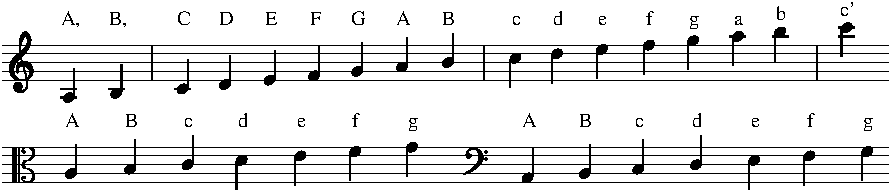
\includegraphics{sample1}
\end{center}

\index{octave}
Note how the clef influences the default octave. 
The default octave can be lowered or raised with the modifier "-8" or
"+8" after the clef in the K: field, e.g. "K:D treble-8". To reset
the octave modifier, use "[K:treble+0]".
\par
\index{accidentals!local} \index{sharp} \index{flat} \index{natural}
The symbols =,\^{ } and \_  are  used  (before  a  note)  to  generate
respectively a natural, sharp or flat. 
Double sharps and flats are available with \^{ }\^{ } and \_\_ respectively.

\subsection{Rhythm}
%-------------------------------------------------------------
\label{sec:MusicRhythm}
\index{note length!specifying}
By default, a letter generates a note with the default length,
specified in the L: info field. If a the letter is followed by /
or /2, the length is halved. If the letter is followed by an integer,
the length is multiplied. Both modifiers can be combined, so that
the multiplier 3/2 produces a dot.

\begin{center}
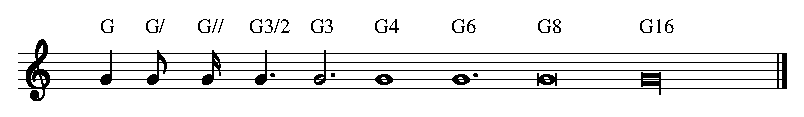
\includegraphics{sample2}
\end{center}

\par
\index{dotted rhythm} For dotted rhythms 
there is a shorthand notation: "\verb$>$" means
`the previous note is dotted, the next note halved' and "\verb$<$" means
`the previous note is halved, the next dotted'. Similarly, "\verb$>>$"
and "\verb$<<$" can be used for double dotting.

\par
\index{rests}
Rests are generated with a {\it z} and can be modified in 
length  in exactly the same way as notes can.

\begin{center}
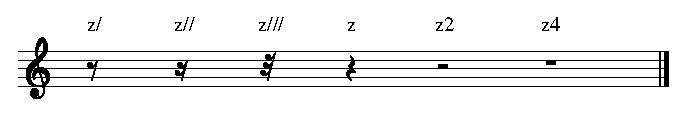
\includegraphics{sample3-edited}
\end{center}

\index{rests!invisible}
Invisible rests are generated with a {\it x}. These count like regular 
rests, but they are not printed. This can be useful in multistave 
music, eg. if one voice has a longer pickup than another voice.
\par
\index{rests!multi bar}
Multi bar rests are generated with a capital {\it Z} followed by the
number of bars. When using bar numbering (command line option ``-k'' or
format parameter {\it \%\%barnumbers}), abctab2ps takes care of multi bar
rests.

\par
\index{triplets} Triplets can be simply coded with the notation "(3abc".
Similarly, "(2ab" makes a duplet, "(4abcd" a quadruplet, etc., 
up to "(9". The musical meanings are:
\begin{center}
\begin{tabular}{|l|l|} \hline
Notation & Meaning \\ \hline
 (2 & 2 notes in the time of 3 \\ \hline
 (3 & 3 notes in the time of 2 \\ \hline
 (4 & 4 notes in the time of 3 \\ \hline
 (5 & 5 notes in the time of n \\ \hline
 (6 & 6 notes in the time of 2 \\ \hline
 (7 & 7 notes in the time of n \\ \hline
 (8 & 8 notes in the time of 3 \\ \hline
 (9 & 9 notes in the time of n \\ \hline
\end{tabular}
\end{center}
If the time signature is compound (3/8, 6/8, 9/8, 3/4, etc.) then
{\it n} is three, otherwise {\it n} is two.

\index{tuplets}
More general tuplets can be specified using the syntax {\it (p:q:r}
which  means `put {\it p} notes into the time of {\it q} for the next {\it r}
notes'. If {\it q}  is not given, it defaults as above. If {\it r} is not
given,  it  defaults  to {\it p}.  For example, "(3:2:2" is equivalent to
"(3::2" and "(3:2:3" is equivalent to "(3:2", "(3" or even 
"(3::". This
can  be  useful  to  include  notes of different lengths within a
tuplet, for example "(3:2:2G4c2" or "(3:2:4G2A2Bc" and also describes
more precisely how the simple syntax works in cases like "(3D2E2F2"
or even "(3D3EF2". The number written over the tuplet is {\it p}.

\index{stemless notes} \index{chant notation}
The notation of nonmetric music like plainchant requires {\it stemless notes}.
These can be enforced with the format parameter {\it \%\%nostems}.
Note that notes still have lengths, so that it is in principle possible
to notate nonmetric music with more than one part (like medieval organa).
To adjust the notes vertically, use invisible rests ({\it x}). Invisible
rests can also be used for separating note groups in monophonic stemless
notation.

\subsection{Bars and repeats}
%-------------------------------------------------------------
\index{bar!lines} \index{bar!invisible} \index{repeats}
Bar lines are specified with a "\verb$|$". abctab2ps does no 
plausibility check whether a bar is over or underfull, so you can 
put bar lines where you please. The following symbols are supported:

\begin{center}
\begin{tabular}{|l|l|} \hline
Notation & Meaning \\ \hline
 \verb$|$ & bar line \\ \hline
 \verb$|]$ & thin-thick double bar line \\ \hline
 \verb$||$ & thin-thin double bar line \\ \hline
 \verb$[|$ & thick-thin double bar line \\ \hline
 \verb$:|$ & left repeat \\ \hline
 \verb$|:$ & right repeat \\ \hline
 \verb$::$ & left-right repeat \\ \hline
 \verb$[|]$ & invisible bar line \\ \hline
\end{tabular}
\end{center}

Invisible bars lines are workarounds if you need labels on the
first bar or put a line break in the middle of a bar.

First and second repeats can be generated with the symbols "\verb$[1$" 
and "\verb$[2$",  e.g.
\begin{quote}
\begin{verbatim}
faf gfe|[1 dfe dBA:|[2 d2e dcB|]
\end{verbatim}
\end{quote}
When adjacent to bar lines, these can be shortened to 
"\verb$|1$" and "\verb$:|2$", but with  regard  to
spaces, i.e. "\verb$| [1$" is legal, "\verb$| 1$" is not.
If you want a dot after the number in first and second repeats, use
the format parameter {\it \%\%endingdots}.

\subsection{Beams, ties and slurs, ligaturae}
%-------------------------------------------------------------
\index{beaming!music}
To group notes together under one beam  they  should  be  grouped
together without spaces. Thus in 2/4, "A2BC" will produce an eighth
note followed by two sixteenth notes under one beam whilst "A2 B C"
will  produce  the  same notes separated. It is possible to put 
rests (z) under a beam, e.g "aza". The beam slopes and the
choice of upper or lower staffs are generated automatically.
\par
\index{ties!music} \index{slurs!music}
You can tie two notes together either across or within a bar with
a  "-" symbol, e.g. "\verb$abc-|cba$" or "\verb$abc-cba$". 
More general slurs can be put in with "()" symbols.  Thus "(DEFG)" 
puts a slur  over  the  four notes.  Spaces within a slur are ok, e.g. 
"(D E F G)", but the open bracket  should  come  immediately  
before a note (and its accents/accidentals,  etc.)  and  the  close  
bracket should come immediately after a note (and its octave 
marker or length).  Thus "(=b c'2)" is correct but ( =b c'2 ) is not.
\par
To abctab2ps, slurs outside chords and slurs within chords are 
different kinds of animals. A slur outside of chord brackets always
applies to the top notes of the enclosed chords and it may span
several notes. A slur within chord brackets however must be 
closed in the immediately following chord. E.g. in order to
tie the top note of a chord to the next single note, you may write
"([afd] b)" or "[(afd] [b)]", but not "[(afd] b)" (in the last
version, the slur is opened inside chord but closed outside which
is not allowed).
\par
\index{ligatura}
In transcriptions of mensural notation into common music notation
{\it ligaturae} are often indicated by square brackets. This is possible
with the pseudocomment {\it \%\%slurisligatura}, which prints ligatura
brackets instead of slurs. Note that this only applies to slurs outside
chords and not to ties.

\subsection{Graces and decorations}
%-------------------------------------------------------------
\index{graces} \index{trill} \index{staccato} \index{appoggiatura}
\index{accacciatura}
\index{bow marks} \index{accents!music} \index{fermata}
\index{segno} \index{coda} \index{breath mark} \index{decorations!music}
Grace notes can be written by enclosing them in curly braces (\verb${}$):

\begin{center}
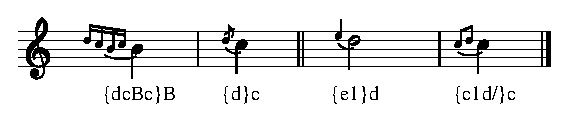
\includegraphics{sample4a}
\end{center}

The first two examples show the meaning of grace notes according to the 
abc standard, which specifies that grace notes have no explicit time values
and the following meaning:
\begin{itemize}
\item A single grace note is an accacciatura
  (see the second example above). In {\em abctab2ps}, the stroke through
  the flag can optionally be suppressed with the format parameter 
  {\em \%\%nogracestroke}.
\item Multiple grace notes are drawn as beamed sixteenth notes.
\end{itemize}
This does not allow for the notation of long appoggiaturas. To overcome this
limitation, {\em abctab2ps} allows for a length specifier in the grace notes
(see the third example above).
The length applies to all grace notes within the same pair of braces; when 
more than one length is specified, the last length holds (see the last example
above).
\par
When the following note is a chord, appogiaturas and accacciaturas
are tied to the first note given in the chord.
\par
Other decorations are indicated either by a magic character (e.g. "T" for a
trill) or by their name in exclamation marks (e.g. "!trill!").
The decoration signs must appear immediately before a note, e.g.
"TG" or "!trill!G" for a trill above middle G. If notes are grouped in chords,
the decoration sign must appear outside and immediately before the chord.
abctab2ps currently supports the following decorations:

\begin{center}
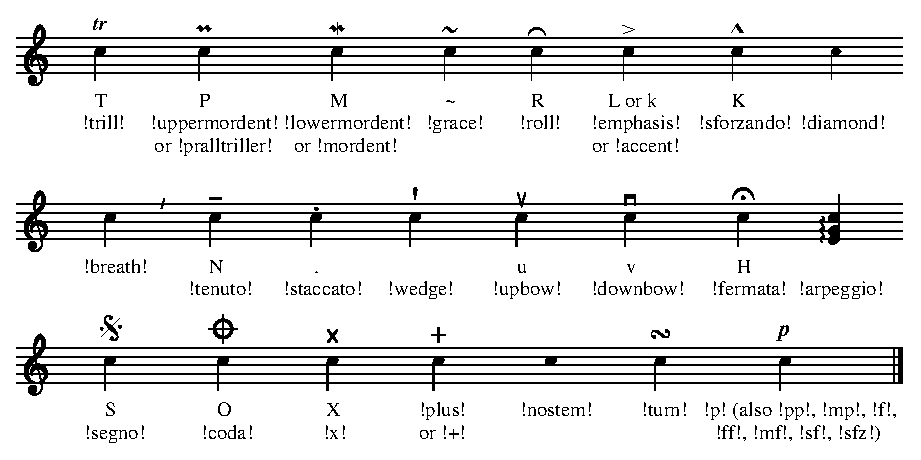
\includegraphics{sample4b}
\end{center}


\subsection{Chords}
%-------------------------------------------------------------
\index{chord} \index{unison}
Chords (i.e. more than one note head on a  single  stem)  can  be
coded  with brackets ([]) around the notes, e.g. "[CEGc]" produces the
chord  C  major.  They  can  be  grouped   in   beams,   e.g.
"[d2f2][ce][df]" but there should be no spaces within a chord.
A chord with two identical notes makes a unison (one head
with stems going both up and down), eg: "[AA]".
\par
\underline{Important notice:} The old style chord notation with
plus signs, eg. "+ac+", which was an undocumented non standard abc 
feature of {\it abc2ps} is no longer supported in abctab2ps.
\par
The abc notation formally permits notes with different durations 
on the same stem: "[a/bc2]" and so on. However, abctab2ps assigns all
notes in a chord the duration of the first note in the bracket.
If you are looking for {\it polyphonie}, see the remark on 
\hyperref{abcm2ps}{abcm2ps in section }{}{sec:PolyphonicMusic}.
\par
Slurs and ties within chords are possible:
\begin{quote}
\begin{tabular}{ll}
 \verb$[(a(b] [c)d)]$ & slurs a to c, b to d \\
 \verb$[a-b] [ac]$    & ties a to a \\
\end{tabular}
\end{quote}

%-------------------------------------------------------------
\section{Text}
%-------------------------------------------------------------
In the tune body, there may be three different types of text:
\begin{itemize}
\item text above the staff (bar labels, guitar chords, bass figures...)
\item text below the staff (lyrics)
\item free text between staffs (stanzas, remarks...)
\end{itemize}
\index{umlauts} \index{accents!text}
Any text may contain characters with dieresis (umlauts) or accents 
in IsoLatin1 decoding. If you are using a different character set
you can emulate these characters with Tex-style escape sequences:
\begin{quote}
\begin{tabular}{ll}
\verb$\'e$ & acute accent: \'e \\
\verb$\`e$ & grave accent: \`e \\
\verb$\^e$ & circumflex accent: \^e \\
\verb$\"e$ & dieresis: \"e \\
\verb$\ss$ & sz (obsolete): \ss \\
\verb$\o \O$ & o slash: {\o} {\O} \\
\verb$\aa \AA$ & a ring: {\aa} {\AA} \\
\verb$\ae \AE$ & ae ligatura: {\ae} {\AE} \\
\verb$\cc \cC$ & c cedilla: \c{c} \c{C} \\
\verb$\~n \~N$ & n twiddle: \~n \~N \\
\end{tabular}
\end{quote}

\subsection{Text above notes and bars}
%-------------------------------------------------------------
\index{guitar chords!music}
Guitar chords can be placed over a note or rest by setting the
chord in double quotes ({\tt "}) immediately before the note,
eg. "{\tt "}Am{\tt "}ab c2". Guitar chords are centred above
the note unless they are especially wide.
\par
\index{basso continuo} \index{figured bass}
Figured bass notation can also be achieved with the guitar chord
notation. In order to stack figures, you can use the escape sequence
\verb$\n$ for line breaks, eg. "\verb$"6\n4"$".
Currently up to eight line breaks are supported, which should
be sufficient for all practical purposes. Please note, that abctab2ps
does not automatically add vertical space for guitar chords with
an insane number of line breaks; if the figures interfere
with the preceding stave, you can add extra space with the voice
parameter {\it space}.
\par
It is possible to have more than one guitar chord over one note. In that
case the guitar chords are equally spaced over the width of the note.
This is useful for harmony changes over a long note, as in the following
example:

\begin{center}
\begin{tabular}{l}
\verb$V:1 clef=treble$ \\
\verb$c/A/B/G/ TA>G | G4 ||$ \\
\verb$V:2 clef=bass$ \\
\verb$"7\n#""6\n4"d2 "5\n4""#"D2 | "#"g4 ||$
\end{tabular}
\begin{tabular}{l}
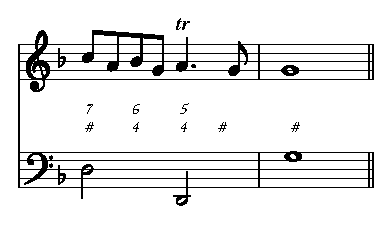
\includegraphics{sample4c}
\end{tabular}
\end{center}

\index{accidentals!in guitar chords}
\index{sharp} \index{flat} \index{natural}
Accidentals in guitar chords can be achieved with the backslash
sequences "\verb$\#$" (sharp), "\verb$\b$" (flat) and
 "\verb$\=$" (natural). Beware that the natural sign is ambiguous
in figured bass notation and is avoided in most historic sources.
It is better to always use {\it flat} for a minor interval and 
{\it sharp} for a major interval; this makes sure that the
figures remain valid in case of transposition.
\par
If you do not like the default gchordfont {\it Helvetica}, you can 
set it with {\it \%\%gchordfont}. A nice font for continuo figures is
{\it ZapfChancery-MediumItalic}.
\par
\index{bar!labels}
\index{bar!decorations}
\index{bar!invisible}
\index{bar numbers!manual}
\index{bar numbers!automatic}
Bar labels like large letters A, B, C...
usually mark specific points in the music. They are coded in 
a syntax similar to guitar chords, but placed before
a bar line instead of a note or rest. For instance
"\verb$| abcd "A"| ABCD |$"
places the letter A over the second bar line.
Just in case somebody wants a label on the first bar
(which is often not preceded by a bar line), the 
symbol \verb$[|]$ means an invisible bar line. When a label is on the last
bar in a line, it is moved to the beginning of the next line.
\par
Although bar numbers can also be written manually over bar lines,
it is more convenient to use abctab2ps' command line option
-k or the pseudocomment {\it \%\%barnumbers} for automatic bar numbering.
\par
Decoration signs are also allowed on bar lines. Although this does not
make much sense for decorations like {\it !trill!} or {\it !mordent!} it
is useful for {\it !segno!} and {\it !coda!}.

\subsection{Lyrics}
%-------------------------------------------------------------
\index{lyrics}
Aligned lyrics under the staff are specified using a line directly
below the staff, starting with "w:". For example:
\begin{quote}
\begin{verbatim}
edc2 edc2 |
w: Three blind mice, three blind mice
\end{verbatim}
\end{quote}
Each blank-delimited word in the w: line is associated with
one note, in sequence. The following special symbols are available
to modify this behaviour:
\begin{quote}
\begin{tabular}{lp{12cm}}
\verb$*$ & skips one note (melisma)\\
\verb$-$ & split a word into two syllables, associated with two notes,
      with '-' drawn between them \\
\verb$|$ & tabs forward to the next bar line.\\
\verb$~$ & is drawn as a space, but contracts words to be written under
      one note. That is, "\verb$hey~ho$" gives two words under one note. \\
\verb$_$ & draws a thin underscore from the previous note to this one. \\
\end{tabular}
\end{quote}
For more than one line of lyrics, just use several w: lines.
To draw a '-' without breaking the word there, escape it as 
"\verb$\-$".
\par
Note that "\verb$\\$" in the abc music line defines a 
staff break. This is
useful when typesetting vocals, because it is tedious to split
the line explicitly when shifting a staff break about when there
are lines with vocals.
\par
If a word starts with a digit, this is interpreted as numbering of a
stanza and is pushed forward a bit. In other words, use something like 
"\verb$w: 1.~~Three blind mice$" 
to put a number before "Three".

\subsection{Free text}
%-------------------------------------------------------------
\index{stanzas} \index{comments!pseudo (\%\%)}
Free text between the music can be inserted either with
W: lines (capital "W" versus lower "w" for lyrics) or with 
{\it pseudo comments} (a line starting with \%\%) in two different ways. \\
First:
\begin{quote}
\begin{verbatim}
%%text This text line is left aligned.
%%center This text line is centered.
%%right This text line is right aligned.
\end{verbatim}
\end{quote}
writes one line into the output. The alignment is given by the
pseudo comment.\\
Second:
\begin{quote}
\begin{verbatim}
%%begintext
%%First line of text
%%Second line
%%And yet another line.
%%endtext
\end{verbatim}
\end{quote}
will write a block of several lines. To avoid conflict with other
programs, the text lines themselves are (optionally) prefaced with 
\%\%.
\par
The statement "\%\%begintext" may have a parameter to determine 
how the output is done, namely: 
\begin{quote}
\begin{tabular}{ll}
\%\%begintext obeylines &  keeps lines as they are (default) \\
\%\%begintext ragged    &  puts in own line breaks to fill the line \\
\%\%begintext align     &  puts in own breaks and aligns right margin \\
\%\%begintext skip      &  skips the whole block, no output \\
\end{tabular}
\end{quote}
For "ragged" and "align", the program has to estimate the number of
lines needed in the current font, since the typesetting is done
using the Postscript "widthshow" operator by the printer. 
The estimate should be reasonably reliable for Times-Roman, but might 
be more dodgy for some other fonts. Also, note that the Ghostview fonts 
can be quite different than the fonts used by the printer.
Strangely, a 13pt font can be smaller than a 12pt font.
\par
An empty line in a block ends a paragraph (see parskipfac below).
In any case, \verb$\\$ can be used in a line of text to 
add line breaks. Thus, two centred lines result from this:
\begin{quote}
\begin{verbatim}
%%center First line\\second line
\end{verbatim}
\end{quote}
As with the other pseudo comments (see section {\it Format fine tuning}), 
the text is associated with a specific tune if it is within that tune's block.
In that case, it will only be printed if that tune is selected. 
If the text is outside all tune blocks, it will always be printed.
The exception is if the command line flag -E is used to to make a separate 
EPS file for each tune. In this case all text outside the blocks is ignored.
\par
To learn how the font for text output is changed, see the section
{\it Format fine tuning}.

%-------------------------------------------------------------
\section{Scores}
%-------------------------------------------------------------

\subsection{Multi stave music}
%-------------------------------------------------------------
\label{sec:MultiStaveMusic}
\index{voices}
abctab2ps supports multi stave music (scores). There are two different
ways for the notation of scores. You can either define the different
voices in V: lines at the end of the header just before the first music
line and use inline V: references "[V:...]" to associate music lines 
with specific voices, as in the following example:

\begin{quote}
\begin{verbatim}
X:1
T:Sonata II
C:B. Marcello, 1712
M:C
L:1/8
K:DDorian
%
V:F clef=treble    name=Flauto space=+5pt
V:B clef=bass      name=Basso  
%
Q:"Adagio"
[V:F] ad fe/d/ eA z A | dd d/e/f/g/ aA z a | 
[V:B] d2 d'2 ^c'2 =c'2 | =b2 _b2 aa/g/ fd | 
\end{verbatim}
\end{quote}

Alternatively, you can write all music of a specific voice immediately
after its voice definition. In this notation the above example reads:

\begin{quote}
\begin{verbatim}
X:1
T:Sonata II
C:B. Marcello, 1712
M:C
L:1/8
K:DDorian
%
Q:"Adagio"
V:F clef=treble    name=Flauto space=+5pt
ad fe/d/ eA z A | dd d/e/f/g/ aA z a | 
%
V:B clef=bass      name=Basso  
d2 d'2 ^c'2 =c'2 | =b2 _b2 aa/g/ fd | 
\end{verbatim}
\end{quote}

The syntax of a voice definition is

\begin{quote}
\begin{verbatim}
V: <label> <par1>=<value1> <par2>=<value2>  ...
\end{verbatim}
\end{quote}

where {\it \verb$<$label\verb$>$ } is used to switch to the voice in later 
V: lines. Each {\it \verb$<$par\verb$>$ = \verb$<$value\verb$>$ } pair sets one 
parameter for the current voice. {\it \verb$<$par\verb$>$ } can be any 
of the following parameters or abbreviations:

\begin{center}
\begin{longtable}{|l|l|l|p{7cm}|} \hline
{\bf Parameter} & {\bf Abbrev.} & {\bf Example} & {\bf Description} \endhead \hline
name  &  nm  &  {\tt nm="Violin I"} & 
    This sets the long version of the voice name, to be
    written before the staves at the start of a piece.
    If the string contains \verb$\\$, this is interpreted
    as a line break and the pieces are writen above 
    each other. \\ \hline
sname &  snm &  {\tt snm="Vl. I"} &
    Short version of the name, written before
    subsequent staves. \\ \hline
clef  &  cl  &   {\tt clef=bass} &
    Chooses the clef (treble, alto, or bass).
    It can also be bass+8 and so on. \\ \hline
staves & stv  &  {\tt stv=2} &
      This is the number of staves (starting from the
      current one) to connect by tall vertical bar lines. \\ \hline
brace  & brc  &  {\tt brace=2} &
      This is the number of staves (starting from the
      current one) to be grouped together with a brace.
      When this option is used, the name defined in the
      same V: line is written at the centre of the brace. \\ \hline
bracket & brk  &  {\tt brk=4} &
      The number of staves to be grouped together by
      a bracket. This option does not change the way
      in which the names are written. \\ \hline
space &  spc  &  {\tt spc=40} &
      This defines or modifies the vertical space between
      this staff and the one below it. The space can be
      given in pt (default) or with a unit in the form 
      1cm or 0.4in. Furthermore: if a + or - sign
      comes after the start of the number, the value
      is an increment to be added to or subtracted
      from the default setting. \\ \hline
gchords  & gch  &  {\tt gch=0}  &
      This controls whether any guitar chords 
      embedded in the current voice are actually written.
      True/false are specified as for the \%\% formats. \\ \hline
stems &  stm  &  {\tt stems=up} &
      This is parsed but not yet used in the program. \\ \hline
octave &  &  {\tt octave=-2} &
      Silently ignored by abctab2ps for compatibility with abc2midi. \\ \hline
\end{longtable}
\end{center}

The various settings (key, default length, etc) are 
maintained for each voice separately.
Guitar chords, first and second endings, and line breaks are 
taken from the top voice only. Vocals can be set under each
voice separately.

\subsection{Polyphonic music}
%-------------------------------------------------------------
\label{sec:PolyphonicMusic}
\index{polyphonie} \index{abcm2ps}
More than one voice on a single stave (polyphonie) is
currently not supported by abctab2ps. However, there is Jean F. Moine's
version of abc2ps named {\it abcm2ps} which handles up to two voices
per stave. This does not sound too exciting, but if you consider that 
each voice can consist of chords, you will realize that almost all 
kind of music can be written in two voices.
\par
In abcm2ps, a pseudo comment of the form
\begin{quote}
\begin{verbatim}
%%staves <definition>
\end{verbatim}
\end{quote}
determines on which staves the voices go. 
{\it \verb$<$definition\verb$>$ } must contain all the voice names with any
pair of "[]", "\{\}" and "()":
\begin{itemize}
\item when not enclosed by special characters, the voices go on separate
  staves.
\item when enclosed by brackets "[]", a bracket is displayed at the 
  beginning of each line.
\item when enclosed by braces "\{\}", the voices go on a single couple 
  of staves (keyboard score). There cannot be more than 4 voices between 
  the braces.
\item when enclosed by parenthesis "()", the voices go on the same staff (no
  more than two voices).
\end{itemize}
When this pseudo comment appears inside a tune, the postscript generation
is restarted as if there was a new tune.
\par
Since abcm2ps is based on an older version of abc2ps, it only accepts
the voice parameters {\it clef}, {\it name} or {\it nm}, {\it snm}.
The other definitions are ignored.

%-------------------------------------------------------------
\section{Tablature}
%-------------------------------------------------------------
\index{lute tablature} \index{guitar tablature}
\index{banjo tablature} \index{ukulele tablature} \index{german tablature}
\index{clef!possible values}
Lines of lute or guitar tablature are distinguished from music lines 
by the particular clefs {\it frenchtab, french4tab, french5tab, 
italiantab, italian7tab, italian8tab, italian4tab, italian5tab,
spanishtab, guitartab, spanish4tab, spanish5tab, banjo4tab, ukuleletab, 
germantab, neapoltab} or {\it banjo5tab}. Like usual clefs, 
they can be specified in the K: field or in the clef parameter of 
a voice definition.
The different clefs specify the following types of tablature:

\begin{description}
\item[frenchtab] In french tablature, the top line stands for the
highest course. The frets at which the courses are stopped are given
by {\it letters}: {\it a} stands for an empty string, {\it b} for the first
fret etc. The letters are printed {\it between} the lines.

\item[french4tab, french5tab] Like {\it frenchtab}, but with four resp.
five tablature lines; one more course than tab lines is supported.

\item[spanishtab, guitartab] In spanish tablature, the top line stands for the
highest course. The frets at which the courses are stopped are given
by {\it numbers}: {\it 0} stands for an empty string, {\it 1} for the first
fret etc. The numbers are printed {\it on} the lines. This tablature 
was used by spanish vihuelists; nowadays it
is quite common as {\it guitar tablature}. Spanish tablature does not
support more than six courses.

\item[spanish5tab, banjo5tab] Similar to {\it spanishtab}, but five tablature
lines; not more than five courses.

\item[spanish4tab, banjo4tab, ukuleletab] Similar to {\it spanishtab}, but 
four tablature lines; not more than four courses.

\item[neapoltab] Similar to {\it spanishtab}, but fret numbers start with 1
instead of 0.

\item[italiantab, italian7tab] In italian tablature, the top line stands 
for the lowest course, which makes this tablature more difficult to learn 
in the beginning. The frets at which the courses are stopped are given
by {\it numbers}: {\it 0} stands for an empty string, {\it 1} for the first
fret etc. The numbers are printed {\it on} the lines. If you want
to notate bourdon strings in italian tablature, you must specify
{\it italian7tab} rather than {\it italiantab}.

\item[italian8tab] Additionally to {\it italian7tab}, stopped courses on
the eighth course are possible. This results in more space between
tabstaff and flags, which might be compensated with a negative value
for \hyperref{\%\%tabflagspace}{{\it \%\%tabflagspace} (see section }{)}{sec:TabFormatParameters}.

\item[italian4tab, italian5tab] Like {\it italiantab}, but with four resp.
five tablature lines; not more than four resp five courses.

\item[germantab] German lute tablature without staff lines and unique
  letters for each fret/course combination. Historically, German tablature
  only supports six courses; higher courses are drawn by abctab2ps like
  in {\em frenchtab}.

\end{description}

\subsection{Course and fret}
%-------------------------------------------------------------
As for music, simultanously plucked strings are written within 
chord brackets "[]". Each position in the bracket marks a specific
course: the first character refers to the first course, the second
character to the second course etc. If the specific course is
unplucked, write a comma ","; is it unstopped write {\it a}; is it
stopped in the first fret write {\it b} etc. If all subsequent courses
are unplucked, you can end the chord.
\par
If a tablature chord consists of only one plucked string the chord
brackets can be omitted. If a chord only contains commas (eg. ``,1'' or
``[,2]''), only the rhythm flag is printed.
\par
The following example shows the notation of a tablature chord and
its output in frenchtab and spanishtab (guitartab):

\begin{center}
\begin{tabular}{lll}
\raisebox{5ex}{\tt [,abc,a] } & 
	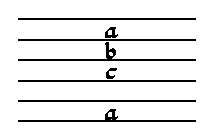
\includegraphics{sample5a} & 
	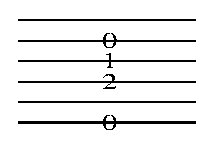
\includegraphics{sample5b} \\ 
\end{tabular}
\end{center}

Remarks:
\begin{enumerate}
\item This "french tablature notation" with letters for the 
frets is the same for {\it all} tablature styles. Depending on the
chosen tabstyle in the clef specification, the output will differ.
Numbers for the frets in the input format cannot be used for two reasons:
\begin{itemize}
\item numbers are already used in the abc language for rhythm
\item frets higher than ten would not be accessible because the numbers
were two characters wide
\end{itemize}
\item In french tablature, the letter "j" is not used. Consequently, 
the letter "k" means the 9th fret etc.
\end{enumerate}
\index{bourdon strings} \index{diapasons}
{\it Bourdon strings} or {\it "diapasons"} are written in braces 
"\{\}". You can use both the ledger line notation for courses 7 to 10
and the number notation; eg. "\{,,,a\}" and "\{10\}" both mean
the tenth course, where the first notation results in an "a" with three
ledger lines and the second results in an "X".
\par
Please note that braces indicate grace notes in music lines. 
Since grace notes are not supported in tablature, braces are abused in 
tablature notation.
\par
\index{german tablature} \index{brummer}
In german lute tablature, the symbols used for the sixth course (``Brummer'')
vary from print to print: some use {\tt A B C D \ldots}, some 
{\tt 1 A B C \ldots} and others {\tt 1 2 3 4 \ldots}, where the numbers
are crossed through. You can choose the style with teh format parameter
{\it \%\%tabbrummer} which can be one of {\it ABC}, {\it 1AB} or {\it 123}.

\subsection{Rhythm}
%-------------------------------------------------------------
\index{note length!tablature}
As for music, the length of a note is specified by a factor with
respect to the default length (L: field). In contrast to music chords
which require the length factor after the {\it first} note in a chord,
tablature chords require the length factor after the {\it last} note
of a chord.
\par
An other important difference concerns the interpretation of chords
without any note length factor. In music, these chords inherit their
length from the default length specified in the L: field. In tablature,
these chords inherit their length from the length of the previous chord
and the rhythm flag is omitted in the printed output (unless you explicitly
ask for a flag on every note with {\it \%\%taballflags}). This means that you 
must specify the length factor "1" if you want a flag above a chord
of the default length.
\par
The shortcuts "\verb$>$" and "\verb$<$" for dotting work like in 
music lines.
\par
The code for triplets and general {\it n}-plets is the 
\hyperref{same as in music,}{same as in music, (see section }{)}
{sec:MusicRhythm}, eg. "(3[a,bc1]cd".
\par
\index{rests!tablature}
There is no consistent way for the notation of rests in tablature:
most historic sources draw a flag with no fret letters, while modern
editions often use modern rest signs. Which rests abctab2ps draws
depends on the 
\hyperref{tabrhstyle}{tabrhstyle (see section }{)}{sec:TabFormatParameters}:
in ``modern'' and ``modernbeams'' style, abctab2ps draws modern style rests;
in all other style
old style rests are drawn. If you need an flag without letter in tabrhstyle
modern, you can use empty chords, eg. ``,1'' or ``[,2]''.
\par
Like tablature chords, rests inherit their length from the previous 
chord or rest and they are only drawn if they explicitly have a rhythm 
factor. Moreover, invisible rests are indicated by {\it x}.

\subsection{Decorations}
%-------------------------------------------------------------
\index{graces!tablature} \index{fermata!tablature} 
\index{appoggiatura!tablature} \index{fingering!right hand}
\index{decorations!tablature}
In music, the abc language only knows graces that affect an 
{\it entire chord}. While this is ok for most decorations, there
are some tablature grace signs (eg. appoggiatura) that apply to a 
{\it single note of a chord}. Thus there are two ways to specify
a tablature decoration:

\begin{itemize}
\item If the magic character (eg. 'H' for fermata) stands {\it outside}
    and {\it immediately before} a chord, the decoration applies to the 
    entire chord. If that decoration usually is associated to a single
    note (eg. appoggiatura or vibrato), it applies to the {\it top note}
    of the chord.
\item If the magic character (eg. '\#' for vibrato) stands {\it inside}
    chord brackets, it applies to the note immediately following that
    magic character. Beware however, that some decorations like fermata 
    cannot be applied to single notes; these decorations are ignored 
    when they appear within chord brackets.
\end{itemize}

The following table lists all graces supported in tablature and whether
they may appear within chord brackets ("applies to chord/note"):

\begin{center}
\begin{longtable}{|l|p{9cm}|l|} \hline
{\bf Input char} & {\bf Meaning} & {\bf Applies to} \endhead \hline
{\tt H} (upper H) & fermata (also \verb$!fermata!$) & chord \\ \hline
{\tt S} (upper S) & segno sign (also \verb$!segno!$) & chord \\ \hline
{\tt O} (upper O) & coda sign (also \verb$!coda!$) & chord \\ \hline
{\tt !p! !pp! !mp!} & dynamic marks (also \verb$!f! !ff! !mf! !sf! !sfz!$) & chord \\ \hline
{\tt .} (dot) & right hand fingering: index finger. \newline
    Is drawn as a single dot under lowest plucked course. & chord \\ \hline
{\tt :} (colon) & right hand fingering: middle finger. \newline
    Is drawn as a double dot under lowest plucked course. & chord \\ \hline
{\tt ;} (semicolon) & right hand fingering: ring finger. \newline
    Is drawn as a triple dot under lowest plucked course. & chord \\ \hline
{\tt +} (plus) & right hand fingering: thumb. \newline
    Representation depends on tablature type: in spanishtab/guitartab
    it is drawn as a plus, in frenchtab or italiantab it is drawn
    as a vertical stroke. & chord \\ \hline
{\tt '} (quote) & an accent after the note. \newline
    In historic sources often used for an appoggiatura or trill
    from above. & note \\ \hline
{\tt X} (upper X) & an 'x' after the note. \newline
    In historic sources often used for a trill or vibrato. & note \\ \hline
{\tt U} (upper U) & an U-shaped arc after the note. \newline
    In historic sources often used for an appoggiatura or trill
    from below. & note \\ \hline
{\tt V} (upper V) & an U-shaped arc below the note. \newline
    The only difference to "U" is that the arc is drawn below
    the tabletter rather than behind. & note \\ \hline
{\tt \#} (sharp) & an '\#' after the note. \newline
    In historic sources used for a trill or vibrato. & note \\ \hline
{\tt *} (asterisque) & an '*' after the note. \newline
    In historic sources used for a vibrato or bass note damping. & 
    note \\ \hline
{\tt T} (upper T) & prints 'tr.' below the chord in italiantab. (also \verb$!trill!$)\newline
    In frenchtab, it is drawn as an accent on the top note of the chord,
    because the 'tr.' symbol would interfere with bourdons. & chord \\ \hline
{\tt L} (upper L) & An oblique line under the note; when applied to
    a chord, it is drawn under the {\it bottom} note of the chord.\newline
    In banjo tablature used to indicate longer notes; in baroque
    french tablature used to indicate an arpeggio. & note \\ \hline
{\tt !strumup!} & An arrow indicating a chord strummed bottom up & 
    chord \\ \hline
{\tt !strumdown!} & An arrow indicating a chord strummed top down & 
    chord \\ \hline
\end{longtable}
\end{center}

\subsection{Text below notes}
%-------------------------------------------------------------
\index{guitar chords!tablature}
The "guitar chord" notation of text enclosed in double quotes
({\tt "}) can be used in tablature too. In tablature however, the
text is printed {\it below} the tablature system rather than {\it above},
because otherwise it would interfere with the rhythm flags.
\par
"Guitar chords" in tablature typically are not used for actual
guitar chord symbols, but for other stuff eg. left/right hand fingering.
Like in music, "guitar chords" can contain line breaks,
indicated by \verb$\n$.

\subsection{Beams, ties and slurs}
%-------------------------------------------------------------
\index{beaming!tablature} \index{ties!tablature} \index{slurs!tablature}
Like in music, ties to the next note can be notatetd with a dash "-"
and more general slurs with parenthesis "()". There is a significant 
difference however: in music, slur bows are also used to indicate 
phrasing and more than one slur can start at a single note. In 
tablature, slur bows always mean "slur" and not more than one slur
may start on a single note, nor may slurs be stacked. Like in music however,
slurs inside and outside of chords are different kinds of animals.
\par
Here are some examples for tablature slurs:
Please note, that the first tie in the second example is not possible in 
music because the opening parenthesis in the chord is not immediately 
closed in the next note.

\begin{center}
\begin{tabular}{l@{\hspace{0.7cm}}l@{\hspace{0.7cm}}l}
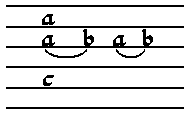
\includegraphics{sample6a} & 
    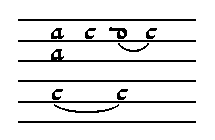
\includegraphics{sample6b} &
    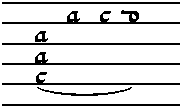
\includegraphics{sample6c} \\[5mm]
{\tt [,a(a,c] [,,b)] (,,a ,,b) } & 
    {\tt [,aa,(c] ,c ([,d,,c)] ,c) } &
    {\tt [,,aa(c] ,a ,c [,d,,y)] }
\end{tabular}
\end{center}

Remarks:
\begin{itemize}
\item The first tie in the second example is not possible in music 
    because the opening parenthesis in the chord is not immediately 
    closed in the next note.
\item In the third example the slur ends on an unplucked course.
    This is achieved by using the letter 'y' (which is not implemented in the
    tablature font) as an anchor for the slur.
\end{itemize}
Beams in the tablature rhythm flags are only drawn when the
rhythm style is set to {\it \%\%tabrhstyle grid} or {\it modernbeams} (see 
\hyperref{Format parameters}{section }{}{sec:TabFormatParameters}).
When this rhythm style is set, the rhythm flags of notes which are
grouped together without white space are connected with beams.
This results in grid shaped rhythm flags as used in some english
16c manuscript sources.

\subsection{Tenuto strokes}
%-------------------------------------------------------------
\index{tenuto strokes}
Tenuto strokes indicating held notes are drawn with \verb$!ten(!$ 
for the start of a tenuto and \verb$!ten)!$ for the end of a tenuto.
These marks are only allowed {\em inside chord brackets}. To let them start
or end on an unplucked course, use the invisible fret symbol {\em y}.
Here are some examples which also show the use of the invisible fret symbol:

\begin{center}
\begin{tabular}{l@{\hspace{0.7cm}}l@{\hspace{0.7cm}}l}
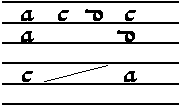
\includegraphics{sample7a} & 
    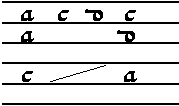
\includegraphics{sample7b} &
    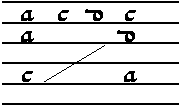
\includegraphics{sample7c} \\[5mm]
{\tt [,aa,!ten(!c] ,c \verb+\+}  & 
    {\tt ,aa,c] [,c,,!ten(!y] \verb+\+} &
    {\tt [,aa,!ten(!c] ,c \verb+\+} \\
{\tt \ \ ,d [,cd,!ten)!a] } &
	{\tt \ \ [,d,,!ten)!y] [,cd,a] } &
	{\tt \ \ [,d,!ten)!y] [,cd,a]}
\end{tabular}
\end{center}


\subsection{Format parameters}
%-------------------------------------------------------------
\label{sec:TabFormatParameters}
\index{comments!pseudo (\%\%)} \index{format file}
Like various aspects of the page layout, some parameters of the
tablature format can be specified via pseudocomments or a format
paramter file. The parameters apply to the entire abc file; if
the same parameter is specified more than once, the last value
overwrites the previous specifications.
\par
In addition to the \hyperref{general parameter format}
{general parameter format (see section }{)}
{sec:LayoutParams}, tablature format parameters can be of
the type {\it keyword} which means a value from a list of special
keywords.
\par
The following parameters are supported:

\begin{center}
\begin{longtable}{|l|l|l|p{7.2cm}|} \hline
{\bf Parameter} & {\bf abctab2ps option} & {\bf Type} & 
	{\bf Description} \endhead \hline
tabfontsize & -tabsize & integer & distance (in pt) between tablature 
    lines and (if tabfontscale=1.0) size of tablature font \\ \hline
tabfontscale & & decimal & scale factor for tablature font.
    If greater than one, tablature letters/numbers are larger than
    the tablature line distance. Can be useful for fonts, which
    are too large or to small (eg. frFrancisque) for your taste. \\ \hline
tabfontfrench & & keyword & font file from which the font for french tablature
    is loaded. (see \hyperref{Tablature Fonts}{section }{}
    {sec:TablatureFonts}) \\ \hline
tabfontitalian & & keyword & font file from which the font for italian 
    tablature is loaded. (see \hyperref{Tablature Fonts}{section }{}
    {sec:TablatureFonts}) \\ \hline
tabfontgerman & & keyword & font file from which the font for german tablature
    is loaded. (see \hyperref{Tablature Fonts}{section }{}
    {sec:TablatureFonts}) \\ \hline
tabaddflags & & integer & how many flags shall be added to tab rhythm signs.
    Eg. a value of 2 means that a quarter note (no flag) in music is 
    printed as sixteenth (two flags) in tablature. Negative values are
    possible but probably not very useful. \\ \hline
tabflagspace & & dimension & additional space between rhythm flags
    and tablature system. Only necessary when the chosen tablature font
    exceeds its bounding box. \\ \hline
tabgchordspace & & dimension & space between gchord text 
    and tablature system. \\ \hline
tabrhstyle & & keyword & style of the rhythm signs. Possible values are
    {\it simple} (headless 16c french style),  {\it grid} (same as simple,
    but with support for beams), {\it modern} (17c french 
    style with heads), {\it modernbeams} (same as modern, but with support
	for beams), {\it diamond} (italian 16c style with diamond
    shaped heads) or {\it none} (no rhythm flags at all). \\ \hline
taballflags & & logical & when true, rhythm flags are printed above all
	notes, even on those without a length factor \\ \hline
tabfirstflag & & logical & when true, rhythm flags are only printed when the
    rhythm changes or after a bar line \\ \hline
tabledgeabove & & logical & when true, ledger lines for french bourdons
    are printed above the note rather than before. \\ \hline
tab8underline & & logical & when true, the 8th course is marked with an
    underline in frenchtab and all following courses are drawn with one
    slash less. \\ \hline
tabbrummer & & keyword & style for the sixth course (``Brummer'') in
    german tablature. Possible values are {\it ABC}, {\it 1AB} or {\it 123}.
    \\ \hline
tabgermansepline & & logical & when false, separator lines between german
    tablature systems are suppressed. \\ \hline
\end{longtable}
\end{center}

Remarks:
\begin{enumerate}
\item The font parameters {\it tabfont*} are {\it global} settings
    which cannot be changed between different tunes (X:) within
    a single abc file.
\item The choice of {\it tabrhstyle} affects the implicit default value of
    {\it tabaddflags}: for "simple" tabrhstyle the latter is 2, otherwise
    it defaults to 0. To override these defaults, simply set {\it tabaddflags}
    explicitly.
\item In case of {\it tabrhstyle none} you might want to set a negative
    value for {\it tabflagspace}.
\end{enumerate}

\subsection{Tablature Fonts}
%-------------------------------------------------------------
\label{sec:TablatureFonts}
\index{fonts!tablature}
abctab2ps reads the font files for tablature letters or numbers
from the directory specified by the environment variable {\it ABCTABFONTS}.
Font file names consist of the name of the composer who used this font
and the prefix {\it fr} (like "french") for letter fonts, {\it it}
(like "italian") for number fonts or {\it de} (like "deutsch") for german
tablature fonts. Font file names are case
sensitive and only the third character is uppercase. Valid font
names are eg.
\begin{quote}
\begin{verbatim}
frFrancisque
itBorrono
deFraktur
\end{verbatim}
\end{quote}
In the abc file you can specify the desired font files with the
pseudocomments {\it \%\%tabfontfrench}, {\it \%\%tabfontitalian} and
{\it \%\%tabfontgerman}, where
the prefix in the font file name optionally may be omitted.
Note that different fonts look best at different sizes: eg.
{\it frFrancisque} should be at least 14pt, while {\it itBorrono}
looks better at 13pt. Thus, when experimenting with different fonts
you should experiment with different values for {\it \%\%tabfontsize}
and {\it \%\%tabfontscale} too.
\par
If you you have some minimal postscript knowledge, you can easily 
define your own tablature font: start with a given font file
and replace the drawing routines for the individual letters or
numbers with your own postscript routines. A font file with the
prefix {\it fr} must define the postscript font {\it FrenchTabfont},
which is used in the drawing routines for french tablature.
A font file with the prefix {\it it} must define the postscript font
{\it ItalianTabfont}, which is used in the drawing routines for
italian and spanish tablature.
\par
The drawing routines
in the default fonts are defined in a 20x20 system, you can change
this with a different {\it /FontBBox} statement. For each character
symbol, you should leave some top space in order to prevent the letters 
from touching each other. Additional bottom space for French fonts is not 
necessary because abctab2ps puts one point space between tablature lines
and the symbols.
\par
In order to make abctab2ps interpret your self defined font correctly,
you must adhere to the following encoding scheme for frenchtab and
italiantab (spanishtab):

\begin{center}
\begin{tabular}{|l|p{9cm}|} \hline
{\bf Character Codes} & {\bf Symbols} \\ \hline
97-119 (ASCII 'a'-'w') & 
    FrenchTabFont: letters for french tablature.\newline
    ItalianTabFont: numbers for italian tablature.\newline
    Please note that 106 ('j') is not used; thus the eigth
    fret is code 105 ('i') and the nineth fret is 107 ('k').\newline
    There is no need to implement all codes; 97-111 ('a'-'o') should
    suffice for almost all purposes. \\ \hline
121 (ASCII 'y') &
    should not be used, because it is reserved as an invisible anchor for
    slurs or decorations on unplucked courses. \\ \hline
68-71 (ASCII 'D'-'G') &
    Numbers '4'-'7' for the french habit of numbering bourdons \\ \hline
72-78 (ASCII 'H'-'O') &
    Numbers '8'-'15' for the italian habit of numbering bourdons \\ \hline
\end{tabular}
\end{center}

If you need special tablature symbols like signs for tenuto signs or damping,
you can use the high code lower case letters 'p'-'w' (112-119) for this
purpose.
\par
For germantab, you must adhere to the following encoding scheme:
\begin{center}
\begin{tabular}{|l|p{10cm}|} \hline
{\bf Character Codes} & {\bf Symbols} \\ \hline
32-97 & symbols for courses 1-5, starting with course 5, fret 0 (c5f0, the
    symbol '1' in germantab) and then c4f0, c3f0, c2f0, c1f0, c5f1, c4f1 etc.
    \newline
    There is no need to implement all codes; 32-87 (up to fret 12) should
    suffice for most purposes. \\ \hline
128-143  & symbols for course 6 (``Brummer'') for {\it \%\%tabbrummer} = 'ABC'
    \\ \hline
144-159  & symbols for course 6 (``Brummer'') for {\it \%\%tabbrummer} = '1AB'
    \\ \hline
160-176  & symbols for course 6 (``Brummer'') for {\it \%\%tabbrummer} = '123'
    \\ \hline
\end{tabular}
\end{center}



\subsection{Unsupported Features}
%-------------------------------------------------------------
The following features are currently not supported in tablature lines:
\begin{itemize}
\item lyrics; is there any need for this feature?
\end{itemize}

%-------------------------------------------------------------
\section{Format fine tuning}
%-------------------------------------------------------------
\label{sec:FormatFineTuning}
\index{comments!pseudo (\%\%)} \index{format file}
Some layout parameter can be set by command line options (see the
man page of abctab2ps or for details), but most are set via
{\it pseudo comments}. Pseudo comments are lines beginning with 
two percentage signs \%\%. The syntax of a 
pseudo comment is
\begin{quote}
\begin{verbatim}
%%<parameter> <value>
\end{verbatim}
\end{quote}
This changes the layout parameter {\it \verb$<$parameter\verb$>$ } to 
{\it \verb$<$value\verb$>$ } in subsequent lines.
\par
These layout settings may also be collected in a {\it format file}
with the extension ".fmt", which can be included with the
command line option -F. This is useful eg. for a songbook because 
the layout of all songs can be maintained in a single file.
Layout parameter in a format file must not start with \%\%.
A line consisting of the word "end" in a fmt file skips the
rest of the file.
\par
To see the settings for all the parameters, use flag -H.
When used in conjunction with other flags such as -p, -P, or -F,
the corresponding parameters are shown. If you redirect the
output to a file and edit out the header line, you immediately
have a prototype fmt file which specifies all the parameters.
\par
There are some parameters which can also be set in the E: info field.
These are
\begin{quote}
\begin{tabular}{ll}
shrink  &  set glue mode to compress \\
space   &  set to natural glue widths \\
stretch &  stretched glue mode \\
fill    &  normal mode to fill staffs \\
break   &  ignore continuations \\
xref    &  write xref numbers to output \\
one     &  write one tune per page. \\
newpage &  start new page for next tune \\
lw {\it ppp}  &  set local staff width to {\it ppp} points.
\end{tabular}
\end{quote}
For example, to output a single tune in a narrower format,
put "E:lw 400" into the header of this tune. If this is put
after the header but within the tune body, only the music is set 
with a different width and the title is written as before.


\subsection{Staff breaking}
%-------------------------------------------------------------
\index{staff break} \index{line continuation}
Generally one line of abc  notation  will  produce  one  line  of
music,  although  if  the music is too long it will overflow onto
the next line. You can counteract this by changing either the note 
spacing with  the  E: field or break the line of abc notation. If, 
however, you wish to use two  lines  of input  to  generate  one  
line  of  music  then simply put a backslash (\verb+\+) at the 
end  of the first line.
\par
The best output is usually obtained if the staff breaks are
chosen explicitly by suitable line breaks in the input file.
In this standard usage, the program tries to set the music as well 
as possible for each line separately. The symbols "*" and "**" at 
the end of a line are ignored, as well as the field "E:" for
the elementary length.
\par
If a line is too long to fit onto one staff, the overhang 
is spilled onto the next staff in this version. This makes it possible 
to get reasonable output even when the input is one long logical line. 
In practice, this is equivalent to automatic line breaking. 
\par
To control line breaking, the following command line options to
abctab2ps are available:
\begin{quote}
\begin{tabular}{lp{10cm}}
 -b  & break at all line ends, even if they end with the
       continuation symbol "\verb+\+". \\
 -c  & consider the input as one long line, ie., implicitly append 
       a backslash to every line of music. \\
 -B {\it n} & try to typeset with {\it n} bars on each line.\\
 -a $\alpha$ & set the maximal amount of permitted shrinking to $\alpha$,
       where $\alpha$ lies between 0 and 1.
\end{tabular}
\end{quote}

\subsection{Fonts}
%-------------------------------------------------------------
\index{fonts!text} \index{fonts!postscript} \index{postscript!standard fonts}
Fonts are specified in pseudo comments of the form
\begin{quote}
\begin{verbatim}
%%<itemfont> <postscript font> <size>
\end{verbatim}
\end{quote}
{\it \verb$<$postscript font\verb$>$ } must be a valid postscript
font. The standard postscript fonts that are supported by all postscript
devices are: {\it AvantGarde-Demi, AvantGarde-DemiOblique,
AvantGarde-Book, AvantGarde-BookOblique,
Bookman-Light, Bookman-LightItalic, Bookman-Demi, Bookman-DemiItalic,
Courier, Courier-Oblique, Courier-Bold, Courier-BoldOblique,
Helvetica, Helvetica-Oblique, Helvetica-Bold, Helvetica-BoldOblique,
Helvetica-Narrow, Helvetica-NarrowOblique, 
Helvetica-NarrowBold, Helvetica-NarrowBoldOblique,
NewCenturySchlbk-Roman, NewCenturySchlbk-Italic, NewCenturySchlbk-Bold,
NewCenturySchlbk-BoldItalic,
Palatino-Roman, Palatino-Italic, Palatino-Bold, Palatino-BoldItalic,
Symbol, Times-Roman, Times-Italic, Times-Bold, Times-BoldItalic, 
ZapfChancery-MediumItalic, ZapfDingbats.}
\par
{\it \verb$<$size\verb$>$ } is the font size in points 
(eg. 14). Note however that the font size (like the size of the music) 
will be effected by the parameter {\it scale} (see next section);
eg. if {\it scale } is set to 0.7 (which is the default) a font size
of 14 will actually result in a $0.7 * 14{\rm pt} \approx 10{\rm pt}$ font. 
\par
{\it \verb$<$itemfont\verb$>$ } specifies the scope of the font like title, guitar 
chords etc. It can be any of the following values (values without
explanation are deemed obvious):
\begin{quote}
\begin{tabular}{ll}
titlefont  & \\
subtitlefont    & \\
composerfont   & \\
partsfont   &   for part labels (P: filed) \\
tempofont   &   for tempo marks (Q: filed) \\
vocalfont   &   for lyrics or vocals under a staff (w: field) \\
gchordfont  &   for guitar chords \\
textfont    &   for text under the tune, or between tunes \\
wordsfont   &   for words under the tune (W: field) \\
voicefont   &   for voice names (V: field) \\
barnumberfont & \\
barlabelfont  & \\
indexfont   &   
\end{tabular}
\end{quote}
In printed music, the bar numbers are often made more visible
by putting a box around them. This is also possible.
In fact, a box can be put around most bits of text by
adding the word "box" to the font specification, e.g.:
\begin{quote}
\begin{verbatim}
%%barnumberfont Times-Italic 11 box
\end{verbatim}
\end{quote}
This can be done for the title, guitar chords, vocals, etc.
To switch on the box without changing the font style and/or size,
the character * can be used, as in:
\begin{quote}
\begin{verbatim}
%%titlefont * * box
\end{verbatim}
\end{quote}
\par
Because ISO fonts are needed for special characters and
accents, all fonts must be known when the header of the PS file
is written. The program tries to be as clever as it can
about this, but a font might be undefined if it is invoked
for the first time further down in a file. For this reason, 
a line like this can be put into the fmt file:
\begin{quote}
\begin{verbatim}
font Palatino-Bold
\end{verbatim}
\end{quote}
or alternatively at the top of the abc file:
\begin{quote}
\begin{verbatim}
%%font Palatino-Bold
\end{verbatim}
\end{quote}
Either of these will define the corresponding ISO font in the header.
To make things even easier, the program always looks for a file
"fonts.fmt" and loads it if it exists. So, the often-used fonts
can be defined there once and for all.

\subsection{Page layout parameters}
%-------------------------------------------------------------
\label{sec:LayoutParams}
\index{layout parameters}
\index{bar numbers!automatic}
\index{ligatura}
Page layout parameter are usually specified by pseudo comments.
Beside dimensionless factors (decimals) or integer values, the parameter 
value can be of the type "logical" or "dimension". Logicals
must be one of {\it 1, yes, true} for "true" or one of {\it 0, no,
false} for "false"; if nothing is specified, this is equivalent to true.
Dimensions can be given in {\it mm}, {\it cm}, {\it in}, or {\it pt}, 
where {\it pt} is the default.
Examples:
\begin{quote}
\begin{verbatim}
%%pageheight 29cm             % height of page
%%staffwidth 5in              % width of staff
%%leftmargin 1.8cm            % left margin
%%titlespace 1cm              % vertical space before the title
%%scale 0.9                   % size of musical symbols
%%staffsep  60pt              % space between staves
\end{verbatim}
\end{quote}
The following table lists all possible parameters and their
equivalent command line option (if there is one). Parameters
without explanation are deemed obvious.
\begin{center}
\begin{longtable}{|l|l|p{1.8cm}|p{7.2cm}|} \hline
{\bf Parameter} & {\bf Type} & {\bf abctab2ps option} & 
	{\bf Description} \endhead \hline
pageheight & dimension & & \\ \hline
staffwidth & dimension & -w & \\ \hline
topmargin & dimension & & \\ \hline
botmargin & dimension & & \\ \hline
leftmargin & dimension & -m & \\ \hline
topspace & dimension & & 
	vertical space at the top of a tune. (see remark 1.) \\ \hline
titlespace & dimension & & 
	space before the title. (see remark 1.) \\ \hline
subtitlespace & dimension & & 
	space before the subtitle. \\ \hline
composerspace & dimension & & 
	space before the composer. \\ \hline
musicspace  & dimension & & 
	space between the composer and the music. \\ \hline
partsspace  & dimension & & 
	space ("up") between the "parts" and the music. \\ \hline
vocalspace & dimension & & 
	space above a line of vocals. \\ \hline
wordsspace & dimension & & 
	space above the words at the end of a tune. \\ \hline
textspace & dimension & -n & 
	space above the text such as history. \\ \hline
gchordspace & dimension &  & 
	space between staff and guitar chords (music only). \\ \hline
staffsep & dimension & -d & 
	separation between staves. One-half of this distance is 
	added above and below each staff. \\ \hline
sysstaffsep & dimension & &
	in multi stave music separation between staves within
	one system. \\ \hline
systemsep & dimension & &
	in multi stave music separation between systems. \\ \hline
stafflinethickness & decimal & &
	thickness of a single music and tablature staffline. \\ \hline
indent & dimension & &
    amount to indent the first staff. Indentation is done at 
    the start of the piece and after a T: field, but not
    after a P: field. \\ \hline
scale  & decimal & -s & 
	symbol size; eg. 1.0 is used in the "pretty" output. \\ \hline
maxshrink & decimal & -a &
	how much to compress horizontally when staff breaks
	are chosen automatically. Between 0 and 1. \\ \hline
strictness1 & decimal & -X &
	strictness for single stave music. \\ \hline
strictness2 & decimal & -X &
	strictness for multi stave music. \newline
	In multi stave music, it is often a good idea to space the notes 
	somewhat more strictly according to their duration than in 
	single stave music. For strictness=1, the spacings for notes
	with short durations is reasonably strictly proportional to
	their duration. For strictness=0, they are spaced about
	equally. Good defaults are strictness1=0.5 and strictness2=0.8. \\ \hline
lineskipfac & decimal & & 
	factor for spacing between lines of text:
	1.0 gives single-space output, 2.0 double etc. \\ \hline
parskipfac & decimal & &  
	similar factor for space after a paragraph of text. \\ \hline
barsperstaff & integer & -B &  
	try to put as many bars per staff. \\ \hline
barnumbers & integer & -k &  
	write bar number every {\it n}-th bar. {\it n=0} writes
    bar number on the first bar in each staff. \\ \hline
barnumberfirst & integer & &  
	Start barnumbering with this number instead of {\it 1}. \\ \hline
landscape & logical & -l & 
	landscape orientation if true \\ \hline
titleleft & logical & & 
	title flushed left if true. \\ \hline
titlecaps & logical & & 
	title in capital letters \\ \hline
musiconly & logical & -M & 
	no lyrics if true \\ \hline
stretchstaff & logical & & 
	stretches underfull staves across page \\ \hline
stretchlast & logical & & 
	stretches last staff if underfull. \\ \hline
writehistory & logical & -n & 
	writes notes, history etc if true. \\ \hline
continueall & logical & -c & 
	continue all lines if true. \\ \hline
breakall & logical & -b & 
	break at all line ends. \\ \hline
oneperpage & logical & -1 & 
	each tune on separate page. \\ \hline
withxrefs & logical & -x & 
	print out X: xref number in title. \\ \hline
squarebrevis & logical & & 
	draw square brevis (\verb$|=|$) instead of round (\verb$|o|$). \\ \hline
slurisligatura & logical & & 
	draw ligatura brackets instead of slurs. \\ \hline
historicstyle & logical & & 
	draw diamond shaped note heads music in order to emulate historic prints.
	Mostly used in connection with {\it nobeams} \\ \hline
nobeams & logical & & 
	do not draw beams in music \\ \hline
nogracestroke & logical & & 
	do not draw stroke through flag of single grace notes \\ \hline
printmetronome & logical & & 
	set to {\it false} or {\it no} when metronome marks in {\tt Q:} fields
	shall not be printed \\ \hline
endingdots & logical & & 
	draw a dot after the number in first/second endings. \\ \hline
meterdisplay & text & &
	for printing different meter specification, eg. {\it \%\%meterdisplay
	3/2=3} will print ``3'' when ``M:3/2'' is given. \\ \hline
\end{longtable}
\end{center}

Remarks:
\begin{enumerate}
\item Usually, one only sees the sum of {\it topspace} and 
{\it titlespace}. However, if text is written preceeding a tune, it
will come after {\it topspace} and before {\it titlespace}.
\item {\it vocalspace, wordsspace} and {\it textspace} count to the top 
of a line of text. That is, the relevant text size (eg. "12pt") is added.
\end{enumerate}

\subsection{Scope of parameters}
%-------------------------------------------------------------
\index{layout parameters!scope}
Generally, layout parameters only affect the current tune in which
they are declared. To make a layout parameter global for all tunes,
declare it before the first X: field or use a separate 
\hyperref{format file}{(see beginning of section }{)}{sec:FormatFineTuning}.
\par
Several parameters (eg. {\it titlefont}, {\it barnumbers},
{\it barnumberfirst}) will only have any effect when they are
declared before the T: field. It is generally the safest
bet to declare format parameters between the X: and T: field.
\par
There is one notable exception from this general scope rules:
\hyperref{tablature font settings}{tablature font settings (see section }{)}{sec:TabFormatParameters}
are global and must be set before or in the first tune.

\subsection{Spontaneous alignment}
%-------------------------------------------------------------
\index{page break} \index{separator line} \index{extra spaces}
If you do not want to change a layout parameter, but simply
want to insert some space or a page break a single position,
you can use the following pseudo comments (all parameters
are of the type "dimension"):
\begin{quote}
\begin{tabular}{lp{10cm}}
\%\%sep  & draws a short centred line as a separator \\
\%\%sep {\it h1 h2 len} & draws a separator of length {\it len} with space 
           {\it h1} above, space {\it h2} below. \\
\%\%vskip {\it h} & adds vertical space of height {\it h} \\
\%\%newpage   & writes a page break
\end{tabular}
\end{quote}

\subsection{Historic layout}
%-------------------------------------------------------------
\index{historicstyle} \index{diamond shaped notes}
If you prefer the look of historic 16th century prints over modern
prints, you can obtain diamond shaped note heads with {\it \%\%historicstyle}
and suppress beaming with {\it \%\%nobeams}. Note that both
parameters only effect music, so that it is still possible to use
grid rhythm flags in tablature in combination with a historic music
layout.

%-------------------------------------------------------------
\section{Other utilities}
%-------------------------------------------------------------

\subsection{abc}
%-------------------------------------------------------------
Although abctab2ps supports some command line options for the
selection of voices or tunes for output, it is often desirable
to write such selections into another abc file. This is achieved
with {\it abcselect}, which is also available from the
\htmladdnormallink{abctab2ps homepage}
{http://www.lautengesellschaft.de/cdmm/}
{\it abcselect} is a platform independent Perl script.
\par
A graphical editor for abc files with syntax highlighting and automatic
invocation of abctab2ps and other third party software (like ghostview)
is available as {\em flabc} from the \htmladdnormallink{abctab2ps homepage}
{http://www.lautengesellschaft.de/cdmm/}.
\par
If you do not like to edit plain text files for the abc input
but prefer some GUI stuff, you can try Jean F. Moine's {\it tclabc}.
As it based upon Tcl/Tk, it runs on almost every platform.
However, {\it tclabc} only supports music, no tablature.

\subsection{Postscript}
%-------------------------------------------------------------
\index{ghostscript} \index{postscript!manipulation tools}
As abctab2ps produces postscript output, you also need some tools 
for processing postscript files (ok, you do not need them necessarily
if you have a postscript printer, but even then some of the following tools 
are useful). If you run Linux, all of these tools should already
be installed on your system; on other operating systems you
possibly need to download, build and install them yourself. 
\par
In order to print postscript files on a non postscript printer,
you need {\it ghostscript}. Ghostcript can not only convert postscript
into almost all printer languages, it even can produce output formats which
may be viewed on the screen. This capability is utilised by the online
previewers {\it ghostview} and {\it gv} (same as ghostview,
but more polished GUI).
\par
There is a number of PS-utilities for manipulating postscript files.
Useful are {\it psselect} (for extracting particular pages, e.g. all
odd or even pages or pages 1 to 7),
{\it psresize} (e.g. for converting EU A4 to US letter and 
vice versa) and {\it psbook} (reorders pages for book printing).
\par
WYSIWIG text processors generally do not allow direct import of plain 
postscript files. In order to display the image in their editor
window, they need a particular version of {\it encapsulated postscript}
named EPSI. EPSI contains a (low quality) bitmap used by the text 
processor for its online preview; on printing the original (high quality)
postscript is used. The tool {\it ps2epsi} converts postscript
to EPSI.

%-------------------------------------------------------------
\section{References and credits}
%-------------------------------------------------------------
\index{abctab2ps homepage}
The latest and greatest version of abctab2ps and its easy to use graphical
user interface ({\em flabc}) is always
avilable from the {\it abctab2ps homepage}, hosted by the German
Lute Society:
\begin{quote}
\htmladdnormallink{http://www.lautengesellschaft.de/cdmm/}
{http://www.lautengesellschaft.de/cdmm/}
\end{quote}
\par
\index{abc2ps}
Since {\it abctab2ps} is built upon {\it abc2ps}, it owes a lot to
Michael Methfessel, the author of {\it abc2ps}. Moreover, significant
parts of this user's guide have been copied from the Readmes of the
abc2ps distribution. The current version of abc2ps is available from
\begin{quote}
\htmladdnormallink{http://www.ihp-ffo.de/\~{}msm/}
{http://www.ihp-ffo.de/\~{}msm/}.
\end{quote}
\par
\index{abcm2ps}
Jean F. Moine's {\it abcm2ps}, which can handle more than one
voice per stave, and the GUI-Editor {\it tclabc}, is available from
\begin{quote}
\htmladdnormallink{http://moinejf.free.fr/}
{http://moinejf.free.fr/}
\end{quote}
\par
\index{abc standard}
The {\it abc} language was originally invented by Chris Walshaw.
On his abc home page
\begin{quote}
\htmladdnormallink{http://abcnotation.org.uk/}
{http://abcnotation.org.uk/}
\end{quote}
you can find links to the official abc standard definition and to a 
wide variety of abc related software. Beware however that {\it abctab2ps}
deviates considerably from the abc standard, because the standard
does not support tablature at all.

\printindex

\end{document}

